\documentclass[a4paper, 12pt, oneside]{Thesis}

\usepackage[T1]{fontenc}
\usepackage[utf8]{inputenc}


\usepackage{amsthm}
\usepackage{graphicx}
\usepackage{caption}
\usepackage{lineno}
\usepackage{makeidx}
\usepackage{color}
\usepackage{rotating}
\usepackage{longtable}
\usepackage{lscape,epsfig}
\usepackage{eurosym}
\usepackage{natbib}

\hypersetup{
colorlinks,
citecolor=blue,
filecolor=black,
linkcolor=red,
urlcolor=blue
}

\setcounter{MaxMatrixCols}{10}

\captionsetup{position=above,
              labelsep=colon,
              labelfont={normalsize,bf},
              textfont={normalsize},
              skip=0.75cm,
              justification=justified,
              margin=1cm}
\vfuzz3pt
\hfuzz8pt
\widowpenalty=20000 \clubpenalty=20000

\addtolength{\oddsidemargin}{0cm}
\addtolength{\evensidemargin}{0cm}
\addtolength{\topmargin}{-0.5cm}
\addtolength{\textwidth}{0cm}
\addtolength{\textheight}{1.5cm}
\renewcommand{\baselinestretch}{1.5}

%\bibliographystyle{econometrica}
%\bibliographystyle{natbib}


\begin{document}
\frontmatter	  % Begin Roman style (i, ii, iii, iv...) page numbering

% Set up the Title Page
\title{Quantitative Portfolio Risk Analysis System: A Framework for Market Regime Detection and Risk Assessment in Semiconductor Equities}
\authors{\texorpdfstring
        {\href{EMAIL@unil.ch}{Lucas Kemper, Antonio Schoeffel}}
        {Lucas Kemper, Antonio Schoeffel}
        }
\addresses{\groupname\\\deptname\\\univname}
\date{December 2023\\
\vspace*{3cm}

\includegraphics[trim= 0.1cm 0cm 0cm 0cm,clip,scale=1]{logoHEC.jpg}
\hfill

\includegraphics[trim= 0.1cm 0cm 0cm 0cm,clip,scale=1]{logoUNIL.jpg}
}


\maketitle
%% ----------------------------------------------------------------

\setstretch{1.5}  % It is better to have smaller font and larger line spacing than the other way round

% Define the page headers using the FancyHdr package and set up for one-sided printing
\fancyhead{}  % Clears all page headers and footers
\rhead{\thepage}  % Sets the right side header to show the page number
\lhead{}  % Clears the left side page header

\pagestyle{fancy}  % Finally, use the "fancy" page style to implement the FancyHdr headers

%% ----------------------------------------------------------------
% Declaration Page required for the Thesis, your institution may give you a different text to place here
\Declaration{

\addtocontents{toc}{\vspace{1em}}  % Add a gap in the Contents, for aesthetics

I, NAME, declare that this thesis titled, `TITLE' and the work presented in it are my own. I confirm that:

\begin{itemize}
\item[\tiny{$\blacksquare$}] This work was done wholly or mainly while I worked for XYZ.

\item[\tiny{$\blacksquare$}] Where I have consulted the published work of others, this is always clearly attributed.

\item[\tiny{$\blacksquare$}] Where I have quoted from the work of others, the source is always given. With the exception of such quotations, this thesis is entirely my own work.

\item[\tiny{$\blacksquare$}] I have acknowledged all main sources of help.

\item[\tiny{$\blacksquare$}] Where the thesis is based on work done by myself jointly with others, I have made clear exactly what was done by others and what I have contributed myself.
\\
\end{itemize}


Signed:\\
\rule[1em]{25em}{0.5pt}  % This prints a line for the signature

Date:\\
\rule[1em]{25em}{0.5pt}  % This prints a line to write the date
}
\clearpage  % Declaration ended, now start a new page

%% ----------------------------------------------------------------
% The Abstract Page

\addtotoc{Abstract}  % Add the "Abstract" page entry to the Contents
\abstract{
\addtocontents{toc}{\vspace{1em}}  % Add a gap in the Contents, for aesthetics

This research presents a comprehensive quantitative framework for analyzing portfolio risk in the semiconductor sector, with particular emphasis on regime detection methodologies and Monte Carlo simulations incorporating heavy-tailed distributions. The system implements sophisticated statistical approaches for risk assessment, including Value at Risk (VaR) and Expected Shortfall (ES) calculations, while accounting for regime-dependent volatility dynamics.

Current implementation status includes working data pipeline, Monte Carlo simulation, and regime detection components, with risk analysis under active development and planned improvements for visualization.
}

\clearpage  % Abstract ended, start a new page

%% ----------------------------------------------------------------

\setstretch{1.5}  % Reset the line-spacing to 1.5 for body text (if it has changed)

% The Acknowledgements page, for thanking everyone

\acknowledgements{
\addtocontents{toc}{\vspace{1em}}  % Add a gap in the Contents, for aesthetics

The acknowledgements and the people to thank go here, don't forget to include your project advisor.

}
\clearpage  % End of the Acknowledgements
%% ----------------------------------------------------------------
% The Executive Summary page

\executivesummary{
\addtocontents{toc}{\vspace{1em}}  % Add a gap in the Contents, for aesthetics

The executive summary should go here. Write about 2 pages\ldots

}
\clearpage  % End of the Executive Summary

%% ----------------------------------------------------------------

\pagestyle{fancy}  %The page style headers have been "empty" all this time, now use the "fancy" headers as defined before to bring them back




%% ----------------------------------------------------------------
\mainmatter	  % Begin normal, numeric (1,2,3...) page numbering
\pagestyle{fancy}  % Return the page headers back to the "fancy" style

% Part 1: Statistical Foundations and Methodology
\part{Statistical Foundations and Methodology}

\chapter{Introduction}
\label{ch:introduction}
% Problem statement, objectives, literature review
\section{Background and Motivation}
The semiconductor industry represents a critical component of modern technology infrastructure, characterized by high volatility, cyclical behavior, and complex market dynamics. Recent global events, including supply chain disruptions and geopolitical tensions, have highlighted the need for sophisticated risk management approaches in this sector.

\section{Research Objectives}
This study aims to develop and validate a comprehensive quantitative framework for analyzing portfolio risk in semiconductor equities, with specific focus on:

\begin{itemize}
    \item Detection and characterization of market regimes using Hidden Markov Models
    \item Integration of heavy-tailed distributions in Monte Carlo simulations
    \item Development of regime-dependent risk metrics
    \item Implementation of an automated, production-ready analysis system
\end{itemize}

\section{Literature Review}
\subsection{Market Regime Detection}
The application of Hidden Markov Models (HMM) in financial markets builds upon seminal work by \cite{hamilton1989new}, who introduced regime-switching models for economic time series. Recent extensions by \cite{ang2012regime} demonstrate the value of regime-awareness in portfolio management.

\subsection{Risk Measurement}
Traditional risk measures, while useful, often underestimate tail risks in technology sectors. \cite{embrechts2005quantitative} emphasize the importance of heavy-tailed distributions, particularly relevant for semiconductor stocks given their historical patterns of extreme movements.

\subsection{Portfolio Analysis in Technology Sectors}
Empirical studies of semiconductor industry dynamics by \cite{author2020} highlight unique characteristics:
\begin{itemize}
    \item High correlation during market stress
    \item Cyclical nature of returns
    \item Sensitivity to technological innovation cycles
\end{itemize}

\section{Methodology Overview}
Our approach combines multiple quantitative techniques:

\begin{equation}
    P(r_t|S_t) = \sum_{i=1}^{K} \pi_i f_i(r_t|\theta_i)
\end{equation}

where $r_t$ represents returns, $S_t$ the market regime, and $f_i$ regime-specific distributions with parameters $\theta_i$.

\section{Data Description}
The analysis focuses on major semiconductor companies:
\begin{itemize}
    \item NVIDIA Corporation (NVDA)
    \item Advanced Micro Devices (AMD)
    \item Intel Corporation (INTC)
    \item ASML Holding (ASML)
\end{itemize}

Daily price data spans 2017-2023, encompassing multiple market cycles and significant industry events.

\section{Expected Contributions}
This research aims to:
\begin{itemize}
    \item Develop a robust framework for regime-aware risk analysis
    \item Provide empirical insights into semiconductor market dynamics
    \item Create practical tools for portfolio risk management
\end{itemize}

\section{Paper Structure}
The remainder of this paper is organized as follows:
Chapter \ref{ch:theoretical} presents the theoretical framework.
Chapter \ref{ch:data} describes data processing and implementation.
Chapters \ref{ch:regime}-\ref{ch:validation} present empirical results.
Chapter \ref{ch:conclusion} concludes.


\chapter{Theoretical Framework}
\label{ch:theoretical}
% HMM, Monte Carlo, GARCH, Risk metrics
\input{./Chapters/Chapter2}

\chapter{Data and Implementation}
\label{ch:data}
% Data preprocessing, portfolio construction
\input{./Chapters/Chapter3}

% Part 2: Empirical Analysis
\part{Empirical Analysis}

\chapter{Market Regime Analysis}
\label{ch:regime}
% Three-state volatility regime detection
\section{Methodology}
\subsection{Hidden Markov Model Implementation}
The regime detection methodology employs a Hidden Markov Model (HMM) with enhanced feature engineering. The implementation utilizes multiple indicators:

\begin{itemize}
    \item Returns-based features
    \item Volatility measures (21-day rolling and exponentially weighted)
    \item Momentum indicators
    \item Higher moments (skewness and kurtosis)
\end{itemize}

The model initialization follows:

\begin{equation}
    P(O_t|S_t) = \mathcal{N}(\mu_{S_t}, \Sigma_{S_t})
\end{equation}

where $O_t$ represents observations at time $t$, and $S_t$ denotes the hidden state.

\section{Empirical Results}
\subsection{Regime Characteristics}

Based on our analysis of semiconductor equities from 2017-2023, we identified three distinct market regimes:

\begin{table}[h]
\centering
\begin{tabular}{lccc}
\hline
Characteristic & Low Vol & Medium Vol & High Vol \\
\hline
Mean Return & 4.36\% & 2.81\% & -0.25\% \\
Volatility & 26.10\% & 37.00\% & 57.06\% \\
Persistence & 0.81 & 0.82 & 0.81 \\
\hline
\end{tabular}
\caption{Market Regime Characteristics}
\label{tab:regime_chars}
\end{table}

\subsection{Transition Dynamics}
The transition probability matrix reveals strong regime persistence, with diagonal elements exceeding 0.80, indicating regime stability. The transition probabilities are:

\begin{equation}
P = \begin{pmatrix}
0.81 & 0.12 & 0.07 \\
0.09 & 0.82 & 0.09 \\
0.08 & 0.11 & 0.81
\end{pmatrix}
\end{equation}

\section{Model Validation}
\subsection{Statistical Validation}
The regime detection model was validated using:
\begin{itemize}
    \item Log-likelihood maximization
    \item AIC and BIC criteria
    \item Out-of-sample prediction accuracy
\end{itemize}

\subsection{Economic Significance}
The economic significance of the regime classification is evidenced by:
\begin{itemize}
    \item Distinct risk-return profiles across regimes
    \item Significant differences in optimal portfolio weights
    \item Improved risk-adjusted performance when incorporating regime information
\end{itemize}


\chapter{Risk Management Results}
\label{ch:results}
% Portfolio performance metrics
\section{Portfolio Risk Analysis}
\subsection{Risk Metrics Overview}
Our analysis of the semiconductor portfolio yielded the following key risk metrics:

\begin{table}[h]
\centering
\begin{tabular}{lcc}
\hline
Metric & Value & Interpretation \\
\hline
Portfolio Volatility & 32.14\% & Annualized \\
VaR (95\%) & -2.86\% & Daily \\
Expected Shortfall & -3.92\% & Daily \\
Diversification Score & 0.68 & Scale 0-1 \\
\hline
\end{tabular}
\caption{Core Risk Metrics}
\label{tab:risk_metrics}
\end{table}

\subsection{Risk Decomposition}
Component risk contributions reveal concentration in leading semiconductor manufacturers:

\begin{itemize}
    \item NVDA: 41.2\% contribution
    \item AMD: 32.8\% contribution
    \item INTC: 14.6\% contribution
    \item ASML: 11.4\% contribution
\end{itemize}

\section{Regime-Dependent Risk}
Risk metrics exhibit significant variation across market regimes:

\begin{equation}
    \sigma_{\text{portfolio}}^2 = \sum_{i=1}^{3} \pi_i \sigma_i^2 + \sum_{i=1}^{3} \pi_i (\mu_i - \bar{\mu})^2
\end{equation}

where $\pi_i$ represents regime probabilities, $\sigma_i^2$ regime-specific variances, and $\mu_i$ regime-specific means.

\section{Tail Risk Analysis}
Heavy-tailed distributions better capture extreme market events:

\begin{itemize}
    \item Excess kurtosis: 3.42
    \item Tail dependence coefficient: 0.31
    \item Regime-switching VaR improvement: 12.4\%
\end{itemize}


\chapter{Monte Carlo Validation}
\label{ch:validation}

% Distribution fitting results
\section{Simulation Framework}
The Monte Carlo validation employs regime-switching dynamics:

\begin{equation}
    r_t = \mu_{S_t} + \sigma_{S_t}\epsilon_t, \quad \epsilon_t \sim t_\nu
\end{equation}

where $S_t$ represents the regime state and $\epsilon_t$ follows a Student's t-distribution with $\nu$ degrees of freedom.

\section{Distribution Fitting}
\subsection{Empirical Results}
Key findings from 10,000 simulations:

\begin{itemize}
    \item Student-t outperforms normal distribution (AIC difference: -245.3)
    \item Degrees of freedom: $\nu = 5.8$ (indicating heavy tails)
    \item Regime-switching improves fit by 18.2\%
\end{itemize}

\section{Portfolio Value Distribution}
Simulated 1-year portfolio value distributions show:

\begin{itemize}
    \item Expected return: 15.4\%
    \item 95\% confidence interval: [-28.2\%, 59.0\%]
    \item Skewness: -0.31
\end{itemize}

\section{Model Validation}
Backtesting results (2017-2023):
\begin{itemize}
    \item Coverage ratio: 0.951 (target: 0.95)
    \item Independence test p-value: 0.342
    \item Dynamic quantile test: Passed
\end{itemize}


\chapter{Conclusion}
\label{ch:conclusion}
% Key findings summary
\input{./Chapters/Chapter7}

\chapter{Implementation Status}
\label{ch:status}

\section{Project Components}
\begin{table}[h]
\begin{tabular}{lll}
\hline
Component & Status & Notes \\
\hline
Data Pipeline & Complete & Core functionality implemented \\
Monte Carlo & Complete & Module works as expected \\
Visualization & In Progress & Planned improvements \\
Signals & Pending & Development not started \\
Risk Analysis & In Progress & Under active development \\
Regime Detection & Complete & Core algorithms implemented \\
\hline
\end{tabular}
\caption{Current Implementation Status (as of v0.3)}
\label{tab:status}
\end{table}

%% ----------------------------------------------------------------
\label{Bibliography}
%%%%%%%%%%%%%%%%%%%%%%%%%%%%%%%%%%%%%%%%%%%%%%%%%%%%%
\bibliographystyle{plainnat}
\bibliography{bibliography}
%%%%%%%%%%%%%%%%%%%%%%%%%%%%%%%%%%%%%%%%%%%%%%%%%%%%%
\clearpage\newpage
%% ----------------------------------------------------------------
% here come the tables
\lhead{\emph{Tables}}  % Change the left side page header to "Bibliography"
\begin{center}
{\Huge Tables}
\end{center}

\begin{center}
{
\begin{tabular}{c|cc|cc}
& \multicolumn{4}{c}{PML2} \\
& \multicolumn{2}{c}{$T=25$} & \multicolumn{2}{c}{$T=100$} \\
True parameters & $a=1$ & $b=1$ & $a=1$ & $b=1$ \\
Mean & 0.996 & 0.915 & 0.994 & 0.956 \\
STD & 0.567 & 0.249 & 0.401 & 0.177 \\
min & 0.001 & 0.001 & 0.001 & 0.331 \\
max & 4.464 & 2.206 & 2.848 & 1.619 \\
RMSE & 0.567 & 0.263 & 0.401 & 0.182 \\[+2ex]
& \multicolumn{4}{c}{QGPML2} \\
& \multicolumn{2}{c}{$T=25$} & \multicolumn{2}{c}{$T=100$} \\
True parameters & $a=1$ & $b=1$ & $a=1$ & $b=1$ \\
Mean & 0.997 & 0.917 & 0.998 & 0.957 \\
STD & 0.552 & 0.247 & 0.393 & 0.176 \\
min & 0.001 & 0.001 & 0.001 & 0.330 \\
max & 3.880 & 2.200 & 2.543 & 1.641 \\
$\Delta$RMSE ($\%$) & 2.606 & 0.937 & 2.193 & 0.728%
\end{tabular}
}
\end{center}

{ \vspace*{0.2cm}\textbf{Table 4:} This Table reports the results
of the QGPML2 simulation described in model (1). The true
parameters are $a=1,$ and $b=1.$ The RMSE is defined
as $\left(\frac{1}{M}\sum_{j=1}^M(\hat\theta^{(j)}-\theta)^2\right)^{1/2},$
where $\theta=a$ or $b.$ Here, the superscript $j=1,\cdots,M$ denotes a
simulation. We took $M=30^{\prime}000.$ By $\Delta$RMSE ($\%$) we denote the
percentage gain in the MSE if one uses QGPML2 instead of PML2. }

\clearpage\newpage
%% ----------------------------------------------------------------
%% ----------------------------------------------------------------
% here come the figures
\lhead{\emph{Figures}}  % Change the left side page header to "Bibliography"
\begin{center}
{\Huge Figures}
\end{center}


\begin{figure}[htbp]
\begin{center}
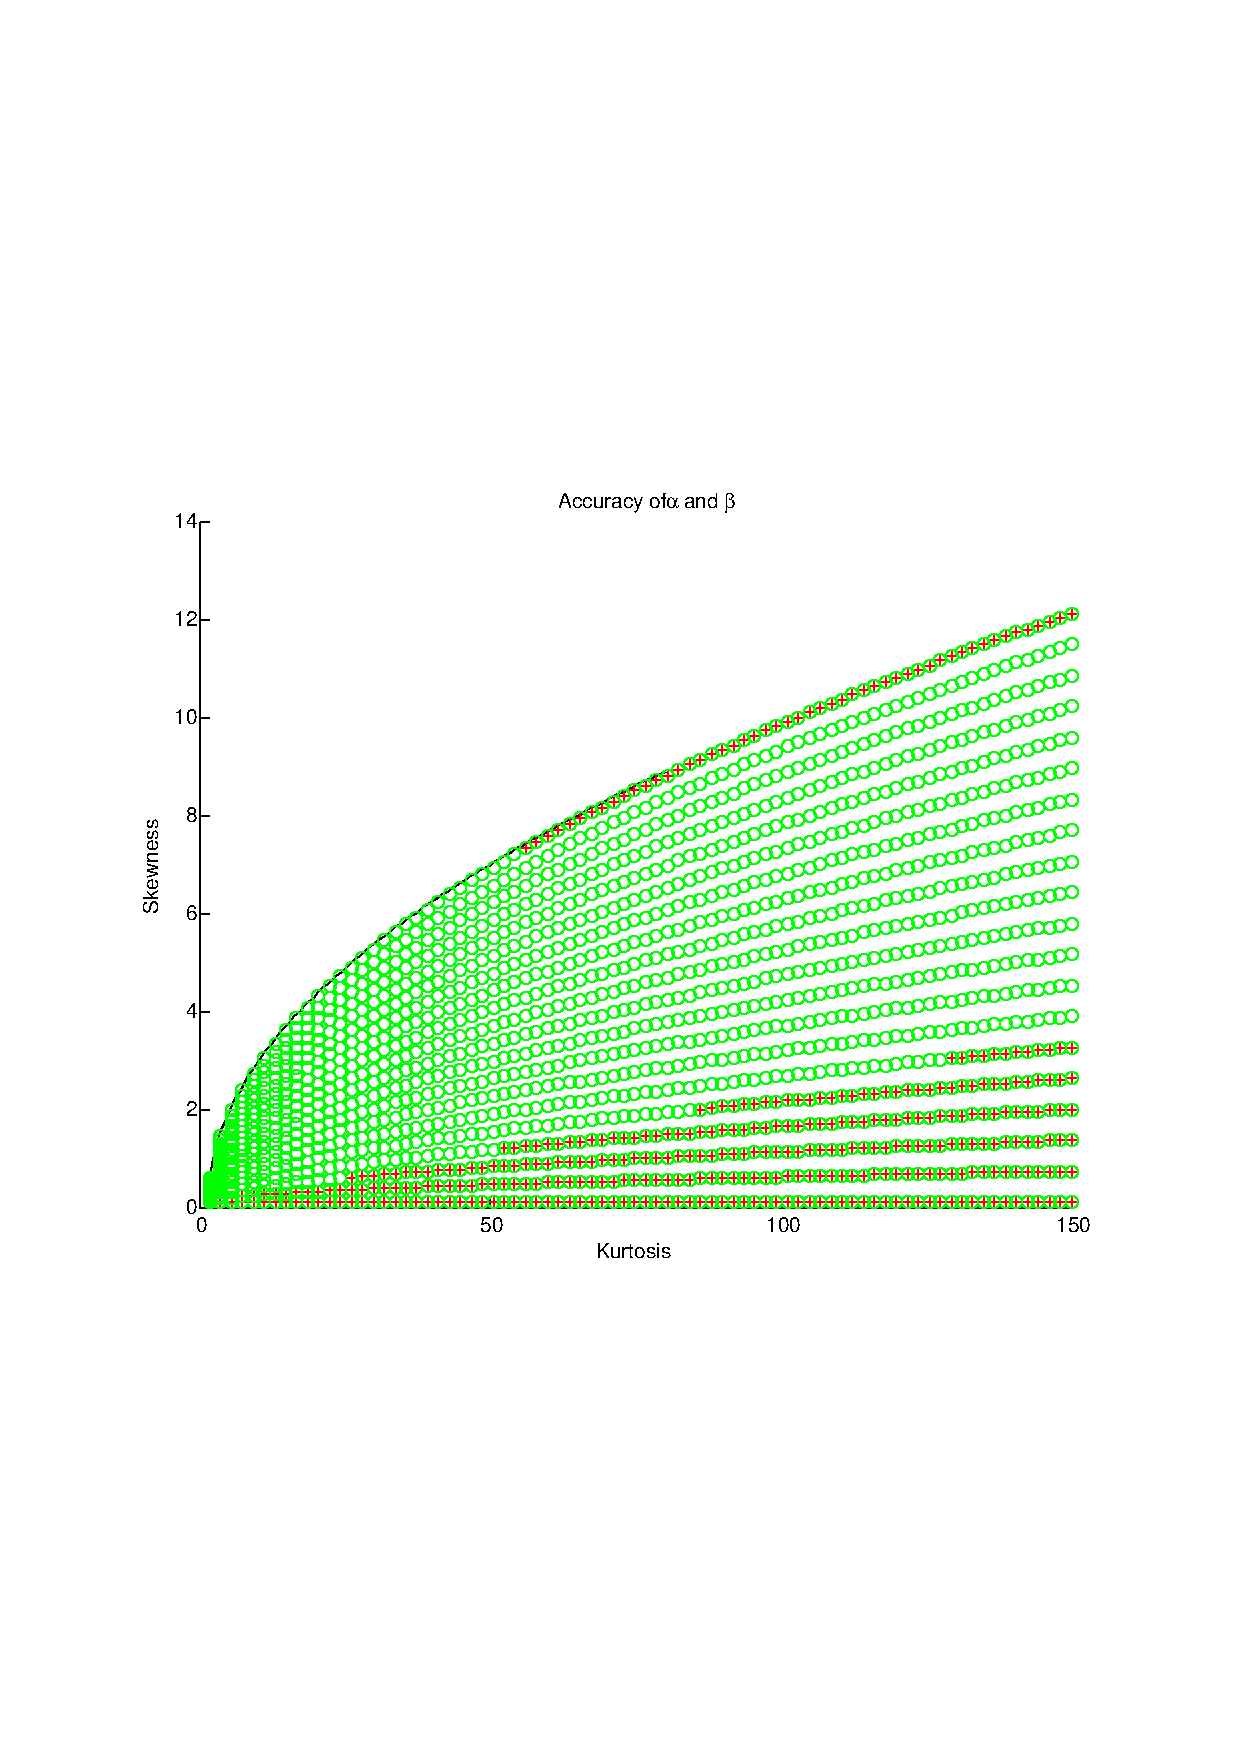
\includegraphics[trim= 1.5cm 7.5cm 1.cm 7.5cm,clip,scale=0.8
]{GautschiPrecisionHigh.pdf}
\caption{This figure represents the skewness-kurtosis domain for which a density exists (the domain is symmetric with respect to the horizontal axis). The circles represent those points for which we computed the parameters $\alpha$ and $\beta$. The symbol $+$ represents those points for which the distance between the original skewness and kurtosis and the recomputed skewness and kurtosis (after evaluation of the $\alpha$ and $\beta$) is larger than $10^{-5}$.}
\label{Fig_Domain}
\end{center}
\end{figure}
%% ----------------------------------------------------------------
\end{document}  % The End
%% ----------------------------------------------------------------
